\documentclass[twoside,openright]{report}
\usepackage[utf8]{inputenc}

\usepackage{graphicx}

\begin{document}


{\Huge Introduction}\\
\rule{12cm}{0.05cm}\\
\newline
\newline
We will begin with axes definition. The line on a graph that runs horizontally (left-right) through zero is called as the X axis. It is used as a reference line so you can measure from it. The X axis goes from $(-\infty, \infty)$. As you go left the value decreases and as you go right the value increases.\\

The line on a graph that runs vertically (top-bottom) through zero is called as the Y axis. The Y axis also goes from $(-\infty, \infty)$. As you go bottom the value decreases and as you go top the value increases.

\begin{figure}[h!]
  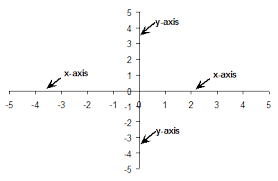
\includegraphics[width=\linewidth]{images.png}
  \caption{X Axis and Y axis.}
  \label{fig:axis1}
\end{figure}
\setcounter{page}{10}
\pagenumbering{arabic}

% page 10 %
\end{document}